\section{Research setup}

An FPGA powered data acquisition board was used as the platform 
for the hardware implementation of digital pulse processing of PMT
signals.
The following subsections describe the system components in detail and
\autoref{fig:system_overview} shows an overview of the test bench.
A 25 kBq $^{137} Cs$ radioactive sample was placed in a plastic V-vial
and used to test the setup.

\begin{figure}[H]
  \centering
  
\includegraphics[width=\linewidth]{media/system_overview.png}
  \caption{HXRM test bench overview}
  \label{fig:system_overview} 
\end{figure}

\subsection{PMT}

Hamamatsu R11265U served as the PhotoMultiplier Tube. 
A 15 mm GPS:Ce scintillator wrapped in aluminium foil was 
coupled directly with the PMT to generate light pulses
from the radiation. The PMT with the scintillator and radioactive material
were placed in a dark 3 mm thick dark iron tube (\autoref{fig:real_emi_tube})
and held together with a custom-designed 3D printed casing (\autoref{fig:real_3dprint}).


\begin{figure}[H]
  \centering
  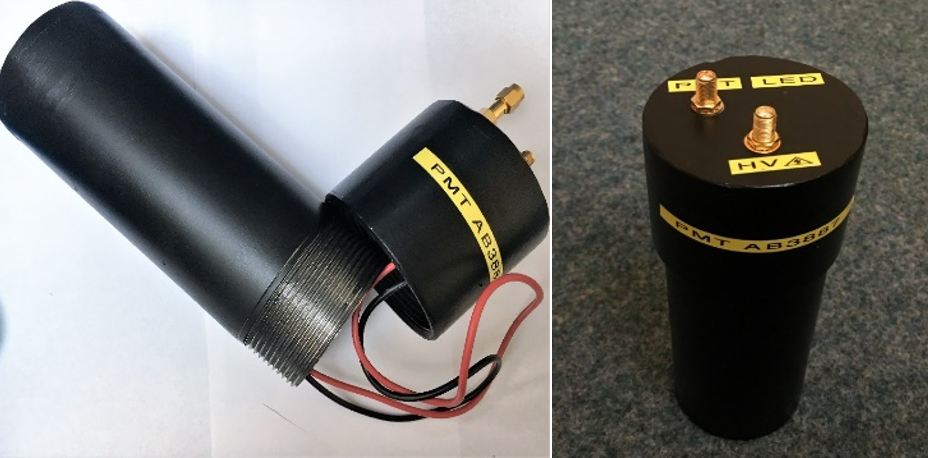
\includegraphics[width=0.75\linewidth]{media/real_emi_tube.png}
  \caption{Exterior tube shielding the system from interference}
  \label{fig:real_emi_tube} 
\end{figure}

\begin{figure}[H]
  \centering
\subfloat[Disassembled coupler and the radioactive sample]{%
  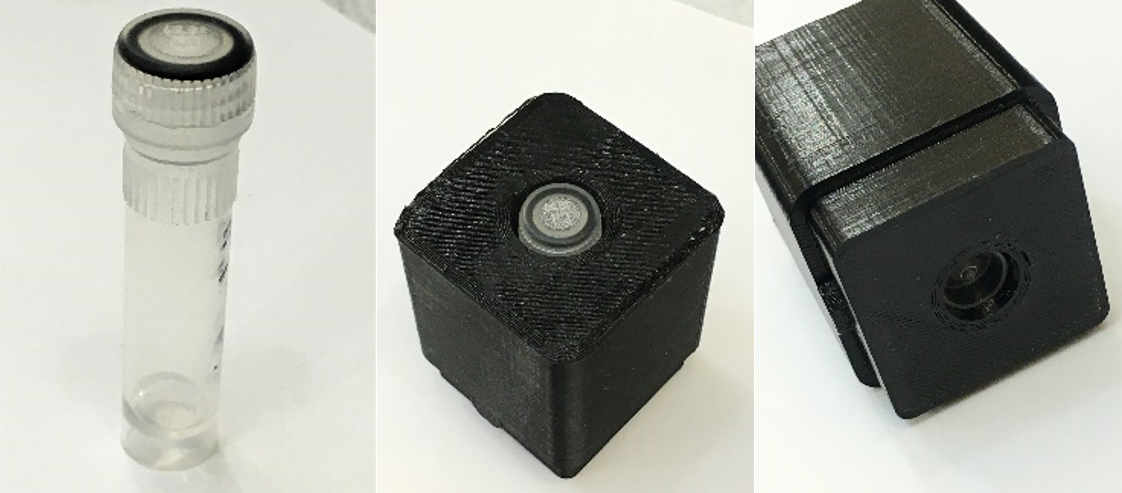
\includegraphics[width=0.7\linewidth]{media/real_cs137.png}
}

  \centering
\subfloat[Assembled coupler]{%
  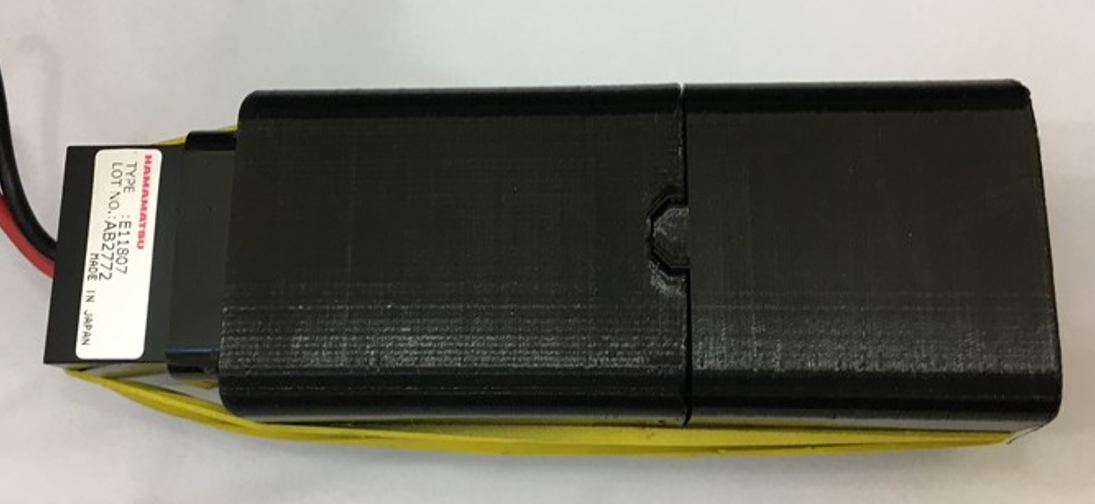
\includegraphics[width=0.7\linewidth]{media/real_3dprint.png}
}
  \caption{Custom 3D printed PMT coupler}
  \label{fig:real_3dprint} 
\end{figure}

\subsection{Preamplifier}

The design of a preamplifier capable of transforming the PMT signal
to satisfy ITER's requirements is a non-trivial task.
No commercially available amplifiers were found
that would satisfy all of the requirements.
Specifically for this project, a custom low-noise preamplifier 
has been developed by Nowakowski et al. and described in another 
paper. 
\cite{low_noise_amplifier_for_pmt}


The PMT-Preamplifier combination used in this work generates pulses that 
fit a single exponential pulse curve with a decay constant of 130 ns.
Bi- and tri-exponential models grant a higher accuracy, but
were found too problematic for real-time processing. 

\subsection{Digitizer board}

To acquire and digitize signals, produced by the PMT and preamplifier
combination, Teledyne SP Devices ADQ14-4C was used. The board was connected
through PCIe 2.0 to the host PC running custom acquisition software.
\begin{table}[H]
\caption{Chosen parameters of ADQ14-4C}
\centering
  \begin{tabular}{l | l}
  {\bfseries Parameter} & {\bfseries Value}\\
  \hline
  \textit {Channel count}             & 4 \\ \hline
  \textit {Sampling rate}  & 1 GS/S \\ \hline
  \textit {Vertical resolution}   & 14 bits\\ \hline
  \textit {Interface}         & PCIe 2.0 x8\\ \hline
  \textit {Max. data transfer rate}         & 3.2 GB/s\\ \hline
  \textit {Internal DRAM memory}      & 2 GB\\ \hline
  \textit {Input range peak to peak}   & 0.2 V - 10 V\\ \hline
  \textit {Number of GPIO ports}         & 12\\ 
  \end{tabular}
  \label{tab:adq14_datasheet}
\end{table}


ADQ14-4C can sample signals from up to 4 channels, each at a maximum
frequency of 1 GHz. It acquires samples with a 14-bit ADC.
The device applies factory calibrated digital gain and shift
to the raw measurements, 
so in order to maintain a higher precision the samples are 
extended to 16 bits representing two full bytes. 
The additional two bits represent the fractional part sometimes
produced by the fractional gain component.


The ADQ14 can operate in both triggered streaming and continuous mode.
In continuous mode samples are constantly gathered and periodically
transferred to the host PC. In triggered streaming a window of samples is 
collected only after a trigger event is detected. This is a basic feature
that allows for some data reduction, as only events of interest have to
be transferred to the host PC. Multiple triggering mechanisms, 
like level, periodic and external are available.


In all modes of operation the device relies on an internal 2 GB DRAM
to act as a FIFO queue for the generated records.
The device relies on Direct Memory Access (DMA) to transfer
data to the host PC. This is a special mode of operation for 
peripheral devices in which a chunk of the computer's memory is
made available to them without the need of CPU brokerage.


Unfortunately, the maximum size of DMA buffers is limited. 
With a sampling speed of a 1 GHz and 2 byte samples, up 
to two gigabytes of data can be generated each second for each
channel that is active. Even with reliance on DMA, maintaining 
a transfer speed this high is problematic. To solve this issue, 
the ADQ14's internal DRAM acts as a buffer.
Records are first stored in the internal DRAM and periodically
transferred to the host PC's RAM whenever DMA buffers become available.
At maximum speed a single channel can, however, still fill the entirety
of this internal buffer in just a second if its contents are not flushed in time.

\subsubsection{Open FPGA design} \label{ssec:adq_devkit}

A crucial feature of ADQ14 is the fact that its core processing
functionality is realised with the use of an on-board FPGA,
more specificaly a Xilinx Kintex 7 K325T. The design of the FPGA
is partially open. Users can implement custom
filtering or data analysis on samples in real time.
This fact is used to implement the real-time pulse processing described in this work.


The firmware is unfortunately not entirely open-source.
Third-party IP cores cannot be distributed to end customers 
and thus user algorithms are limited to two sections called User Logics
as indicated in \autoref{fig:devkit_structure}.
User Logic 1 is a core placed after the ADC samples are subjected to factory
gain, but before the signals are passed on to trigger control.
This enables the implementation of custom triggering logic.

\begin{figure}[H]
  \centering
  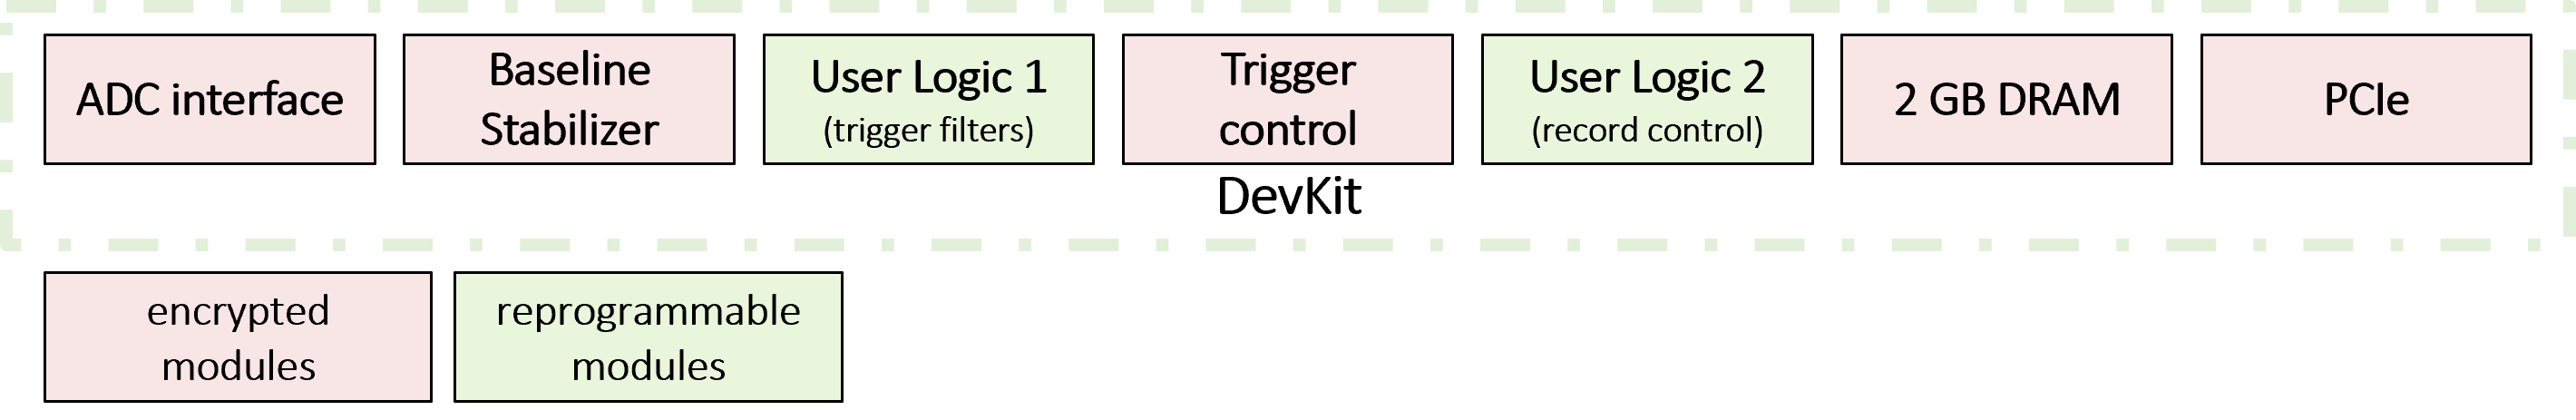
\includegraphics[width=\linewidth]{media/devkit_structure.png}
  \caption{Structure of the ADQ14 DevKit}
  \label{fig:devkit_structure} 
\end{figure}


User Logic 2 is intended to house more complicated logic.
This module has access to the GPIO ports and some metadata
outputs, that can be used to describe the transferred data.
User Logic 2 is located right before the encrypted packet generator
that is responsible for queueing the incoming data in ADQ14's DRAM 
for transfer to the host PC. The packet generator can be partially
controlled from within User Logic 2. Arbitrary data can be injected
in place of the samples for each channel and the size of transferred windows 
can be modified.

\subsubsection{Parallel sampling} \label{sssec:parallel_sampling}

The FPGA is clocked only at 250 MHz which is exactly a quarter of 
the ADC maximum operating frequency. This means that each channel
of the digitizer produces 4 samples on each clock cycle of the 
FPGA. This is a necessary design choice as FPGAs fare better 
at lower clock speeds due to the need of less complex routing
when it comes to connecting the various peripherals and CLBs.


Such design does, however, complicate the implementation of 
Digital Signal Processing. It is especially cumbersome for 
functions that depend on delayed samples.
Accumulators have the need of summing up 4 samples on
each clock cycle instead of one. Complicated operations
like multiplication and division require duplicated logic.
Most functionality has to be properly pipelined to avoid
timing issues in the FPGA design.

\subsection{Host computer}

The host computer was running Red Hat Enterprise Linux 7.
\autoref{tab:pc_specs} lists the computer hardware configuration.
The system configuration was chosen by ITER and is a part of the 
Control, Data Access and Communication Core System (CODAC CS)
\cite{codac}.
\begin{table}[H]
\caption{Hardware configuration of the host PC}
\centering
  \begin{tabular}{l | l}
  {\bfseries Parameter} & {\bfseries Value}\\
  \hline
  \textit {CPU}             & Intel Xeon C5549 \\ \hline
  \textit {Storage}  & Samsung 970 EVO Plus 500 GB \\ \hline
  \textit {Operating System}   & Red Hat Enterprise Linux 7.4\\ \hline
  \textit {GPU}         & NVIDIA GP107 \\ \hline
  \textit {RAM}      & 24 GB DDR3 1333 MHz\\ 
  \end{tabular}
  \label{tab:pc_specs}
\end{table}

